\documentclass[../poma-notes.tex]{subfiles}

\graphicspath{\subfix{../images/}}

\begin{document}

\subsection*{Compact Sets}

\begin{definition}
  By an \textit{open cover} of a set $E$ in a metric space $X$ we mean a collection $\{G_{\alpha}\}$ of open subsets
  of $X$ such that $E \subset \cup_{\alpha} G_{\alpha}$.
\end{definition}

\anote \textit{开覆盖} open cover。

\begin{definition}
  A subset $K$ of a metric space $X$ is said to be \textit{compact} if every open cover of $K$ contains a $finite$
  subcover.

  More explicitly, the requirement is that if $\{G_{\alpha}\}$ is an open cover of $K$, then there are finitely many
  indices $\alpha_1,\dots,\alpha_n$ such that
  \[K \subset G_{\alpha_1} \cup \cdots \cup G_{\alpha_n}\ .\]
\end{definition}

紧性 compactness 这个概念在数学分析中非常的重要,特别是它连接了连续性这个概念(第四章)。

很明显所有的有限集都是紧的。$R^k$ 上存在大类无限紧集将会在 Theorem 2.41 中提及。

我们之前观察到的(Remark 2.29)如果 $E \subset Y \subset X$,那么 $E$ 有可能相对 $Y$ 是开的,而不需要相对 $X$ 是开的。
开这个属性因此取决于 $E$ 所嵌入的空间,对于闭这个属性亦是如此。

\begin{anote}
  \begin{itemize}
    \item 紧集 compact set:任何开覆盖都存在有限的子覆盖。
    \item 若一个集合是紧集,可以称这个集合具有紧性 compact。
    \item 紧性实际上是一种拓扑性质。
  \end{itemize}
\end{anote}

\begin{theorem}
  Suppose $K \subset Y \subset X$. Then $K$ is compact relative to $X$ if and only if $K$ is compact relative to $Y$.
\end{theorem}

凭借这个定理,在许多情况下,我们能够将紧集本身视为度量空间,而无需关注任何嵌入空间。尽管讨论\textit{开}空间,或者\textit{闭}
空间的意义不大(每个度量空间 $X$ 是其自身的一个开子集,以及一个闭子集),但是讨论\textit{紧}度量空间却是很有意义的。

\begin{proof}
  假设 $K$ 是相对 $X$ 紧的,且令 $\{V_{\alpha}\}$ 为相对 $Y$ 是开的集合类,使得 $K \subset \cup_{\alpha} V_{\alpha}$。
  根据 Theorem 2.30,存在若干相对 $X$ 是开的集合 $G_{\alpha}$,使得对于所有 $\alpha$ 有 $V_{\alpha} = Y \cap G_{\alpha}$;
  又因为 $K$ 是相对 $X$ 紧的,我们有
  \begin{equation}
    K \subset G_{\alpha_1} \cup \cdots \cup G_{\alpha_n}
  \end{equation}
  对于一些有限数量索引 $\alpha_1, \dots, \alpha_n$。因为 $K \subset Y$,(22) 意味着
  \begin{equation}
    K \subset V_{\alpha_1} \cup \cdots \cup V_{\alpha_n}
  \end{equation}
  这证明了 $K$ 是相对 $Y$ 紧的。

  相反的,假设 $K$ 是相对 $Y$ 紧的,令 $\{G_{\alpha}\}$ 为 $X$ 开子集的类,其覆盖了 $K$,且令 $V_{\alpha}=Y\cap G_{\alpha}$。
  那么 (23) 将包含一些 $\alpha_1, \dots, \alpha_n$;又因为 $V_{\alpha} \subset G_{\alpha}$,(23) 意味着 (22)。

  证明结束。
\end{proof}

\begin{anote}
  首先是证明 $K$ 相对 $Y$ 紧:假设 $K$ 相对 $X$ 紧。根据条件 $K \subset Y$ 可以设定 ${V_{\alpha}}$ 为 $K$ 在 $Y$ 上的子覆盖,
  那么根据开覆盖的定义有 $K \subset \cup_{\alpha}V_{\alpha}$;利用 Theorem 2.30 -- $Y$ 上的子集 $V$ 当且仅当 $V = Y \cap G$
  且$G$ 为 $X$ 的开集时, $V$ 相对 $Y$ 开,那么对于所有的 $\alpha$ 则有 $V_{\alpha} = Y \cap G_{\alpha}$;根据假设 $K$ 相对
  $X$ 紧,那么在 $X$ 上存在有限的子覆盖,即 $K \subset G_{\alpha_1} \cup \dots \cup G_{\alpha_n}$;而先前的设定的 $V_{\alpha}$
  与 $G_{\alpha}$ 因为子覆盖是有限的,那么可以建立 $V_{\alpha_1}=Y\cap G_{\alpha_1},\dots,V_{\alpha_n}=Y\cap G_{\alpha_n}$
  这样一一对应的关系,对于 $K \subset G_{\alpha_1} \cup \dots \cup G_{\alpha_n}$ 可以在子集符两边做与 $Y$ 的交集,即
  \begin{align*}
    \mathcal{} Y \cap K & \subset Y \cap \left(G_{\alpha_1} \cup \dots \cup G_{\alpha_n}\right)                     \\
                        & \subset \left(Y \cap G_{\alpha_1}\right) \cup \dots \cup \left(Y \cap G_{\alpha_n}\right) \\
                        & \subset V_{\alpha_1} \cup \dots \cup V_{\alpha_n}
  \end{align*}
  又因为 $K \subset Y$ 那么 $Y \cap K = K$,所以上述简化为 $K \subset V_{\alpha_1} \cup \dots \cup V_{\alpha_n}$,也就是说
  $V_{\alpha}$ 是 $K$ 在 $Y$ 上有限的子覆盖,即证明了 $K$ 是相对 $Y$ 紧的。

  其次是证明 $K$ 相对 $X$ 紧:假设 $K$ 相对 $Y$ 紧。令 $\{G_{\alpha}\}$ 为 $K$ 在 $X$ 上的开覆盖子集的类,利用 Theorem 2.30
  有 $V_{\alpha} = Y \cap G_{\alpha}$,那么根据 (23) 可以推导出 (22)。即证明了 $K$ 是相对 $X$ 紧的。
\end{anote}

\begin{theorem}
  Compact subsets of metric spaces are closed.
\end{theorem}

\begin{proof}
  令 $K$ 为度量空间 $X$ 的一个紧子集。我们应该证明 $K$ 的补集是 $X$ 上的一个子开集。

  假设 $p \in X,\ p \notin K$。如果 $q \in K$,令 $V_q$ 与 $W_q$ 分别为 $p$ 与 $q$ 的邻域,它们的半径小于 $\frac{1}{2}d(p,q)$
  (详见 Definition 2.18 (a))。由于 $K$ 是紧的,那么在 $K$ 中存在有限数量的点 $q_1,\dots,q_n$ 使得
  \[K \subset W_{q_1} \cup \cdots \cup W_{q_n} = W\ .\]
  如果 $V = V_{q_1} \cup \cdots \cup V_{q_n}$,那么 $V$ 是 $p$ 的一个邻域,且不与 $W$ 相交。因此 $K \subset K^c$,所以 $p$ 是
  $K^c$ 的一个内点。
\end{proof}

\anote 度量空间的紧子集是闭的;度量空间的紧集都是有界的.

\begin{theorem}
  Closed subsets of compact sets are compact.
\end{theorem}

\begin{proof}
  假设 $F \subset K \subset X$,$F$ 是闭的(相对于 $X$),且 $K$ 是紧的。令 $\{V_{\alpha}\}$ 为 $F$ 的一个开覆盖。如果 $F^c$
  临近 $\{V_{\alpha}\}$,我们得到一个 $K$ 的开覆盖 $\Omega$。由于 $K$ 是紧的,那么存在一个有限的子类 $\Phi$ 覆盖 $K$,也覆盖了
  $F$。如果 $F^c$ 是 $\Phi$ 的一个成员,我们将其从 $Phi$ 中移除并保持 $F$ 的一个开覆盖。综上所述,$\{V_{\alpha}\}$ 的一个有限的
  子类覆盖了 $F$。
\end{proof}

\anote 紧集的子闭集是紧的。

\begin{corollary}
  If $F$ is closed and $K$ is compact, then $F \cap K$ is compact
\end{corollary}

\begin{proof}
  Theorem 2.24 (b) 以及 2.34 展示了 $F \cap K$ 是闭的;由于 $F \cap K \subset K$。Theorem 2.35 展示了 $F \cap K$ 是紧的。
\end{proof}

\anote 闭集与紧集的交集是紧的。

\begin{theorem}
  If $\{K_{\alpha}\}$ is a collection of compact subsets of a metric space $X$ such that the intersection of every finite
  subcollection of $\{K_{\alpha}\}$ is nonempty, then $\cap K_{\alpha}$ is nonempty.
\end{theorem}

\begin{proof}
  从 $\{K_{\alpha}\}$ 中固定一个成员 $K_1$ 并令 $G_{\alpha} = K_{\alpha}^c$。假设 $K_1$ 中没有点属于任何的 $K_{\alpha}$。
  那么集合 $G_{\alpha}$ 形成了 $K_1$ 的一个开覆盖;又因为 $K_1$ 是紧的,存在有限数量的索引 $\alpha_1,\dots,\alpha_n$ 使得
  $K_1 \subset G_{\alpha_1} \cup \cdots \cup G_{\alpha_n}$。但是这就意味着
  \[K_1 \cap K_{\alpha_1} \cap \cdots \cap K_{\alpha_n}\]
  为空,与假设相悖。
\end{proof}

\begin{anote}
  证明中的假设是拿出一个子紧集 $\{K_1\}$ 作为特例,假设其不与任何其他 $\{K_{\alpha}\}$ 相交,那么它则会属于其他 ${K_{\alpha}}$ 并集的
  补集,也就是说后者成为了前者的开覆盖;又因为紧集的性质,$K_1$ 开覆盖的子集是有限的,这意味后者是有限的,即证明中的
  \[K_1 \subset G_{\alpha_1} \cup \cdots \cup G_{\alpha_n}\]
  成立,那么就有
  \begin{align*}
    \mathcal{} K_1 & \not\subset K_{\alpha_1} \cap \cdots \cap K_{\alpha_n} \\
                   & \cap K_{\alpha_1} \cap \cdots \cap K_{\alpha_n}        \\
                   & = \emptyset
  \end{align*}
  与假设相悖。
\end{anote}

\begin{corollary}
  If $\{K_n\}$ is a sequence of nonempty compact sets such that $K_n \supset K_{n+1} \ (n=1,2,3,\dots)$, then
  $\cap_1^{\infty} K_n$ is not empty.
\end{corollary}

\anote
如果 $\{K_n\}$ 是一个非空紧集的数列,使得 $K_n \supset K_{n+1} \ (n=1,2,3,\dots)$,那么 $\cap_1^{\infty} K_n$ 不为空。

\begin{theorem}
  If $E$ is an infinite subset of a compact set $K$, then $E$ has a limit point in $K$.
\end{theorem}

\begin{proof}
  如果 $K$ 中没有点是 $E$ 的极限点,那么每个 $q \in K$ 将会有一个邻域 $V_{\alpha}$,其包含了 $E$ 中至多一个点(命名 $q$,
  如果 $q \in E$)。很明显 $\{V_q\}$ 没有有限子类可以覆盖 $E$;对 $K$ 也是同理,因为 $E \subset K$。这与 $K$ 的紧性相悖。
\end{proof}

\anote
如果 $E$ 是紧集 $K$ 的无限子集,那么 $E$ 在 $K$ 中存在极限点。证明中的\say{$\{V_q\}$ 没有有限子类可以覆盖 $E$}是因为 $E$
是无限子集。

\begin{theorem}
  If $\{I_n\}$ is a sequence of intervals in $R^1$, such that $I_n \supset I_{n+1} \ (n=1,2,3,\dots)$, then
  $\cap_1^{\infty} I_n$ is not empty.
\end{theorem}

\begin{proof}
  如果 $I_n = [a_n,b_n]$,令 $E$ 为所有 $a_n$ 的集合。那么 $E$ 是非空且有上界的(为 $b_1$)。令 $x$ 称为 $E$ 的上确界。
  如果 $m$ 与 $n$ 是正整数,那么
  \[a_n \le a_{m+n} \le b_{m+n} \le b_m \ ,\]
  使得对每个 $m$ 有 $x \le b_m$。很显然 $a_m \le x$,可知对 $m=1,2,3,\dots$ 有 $x \in I_m$。
\end{proof}

\begin{anote}
  证明中所设置的 $m$ 作为增量,记 $m=1,2,3,\dots$,这是为了满足定理中的 $I_n \supset I_{n+1}$。
  \begin{center}
    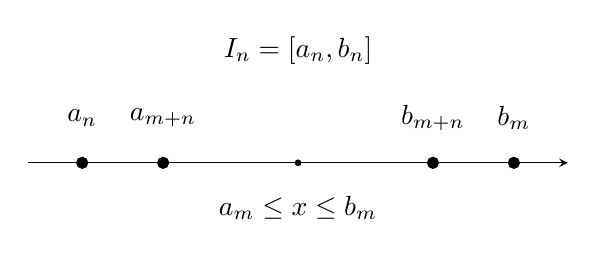
\begin{tikzpicture}
      \begin{axis}[
          xmin=-10, xmax=10,
          axis x line=center,
          hide y axis,
          ymin=-5,ymax=5,
          xtick=\empty,
          xticklabels=\empty,
        ]
        \draw[color=black] (0,2.5) node {$I_n = [a_n, b_n]$};
        \begin{scriptsize}
          \draw [fill=black] (-8,0) circle (2pt);
          \draw[color=black] (-8,1) node {$a_n$};

          \draw [fill=black] (-5,0) circle (2pt);
          \draw[color=black] (-5,1) node {$a_{m+n}$};

          \draw [fill=black] (0,0) circle (1pt);
          \draw[color=black] (0,-1) node {$a_m \le x \le b_m$};

          \draw [fill=black] (5,0) circle (2pt);
          \draw[color=black] (5,1) node {$b_{m+n}$};

          \draw [fill=black] (8,0) circle (2pt);
          \draw[color=black] (8,1) node {$b_{m}$};
        \end{scriptsize}
      \end{axis}
    \end{tikzpicture}
  \end{center}
  集合 $E$ 在最开始有明确的上界,即 $b_1$,随着 $m$ 增加 $a_m \le x \le b_m$ 始终成立。
\end{anote}

\begin{theorem}
  Let $k$ be a positive integer. If $\{I_n\}$ is a sequence of $k$-cells such that $I_n \supset I_{n+1} \ (n=1,2,3,\dots)$,
  then $\cap_1^{\infty} I_n$ is not empty.
\end{theorem}

\begin{proof}
  令 $I_n$ 包含所有点 $\mathbf{x} = (x_1,\dots,x_k)$ 使得
  \[a_{n,j} \le x_j \le b_{n,j} \quad (1 \le j \le k; n=1,2,3,...)\]
  且令 $I_{n,j} = [a_{n,j},b_{n,j}]$。对于每个 $j$,数列 $\{I_{n,j}\}$ 满足 Theorem 2.38 的假设。因此存在实数
  $x_j^*(1 \le j \le k)$ 使得
  \[a_{n,j} \le x_j^* \le b_{n,j} \quad (1 \le j \le k; n=1,2,3,...)\]
  设置 $\mathbf{x^*} = (x_1^*, \dots, x_k^*)$,得 $\mathbf{x^*} \in I_n$ 其中 $n=1,2,3,\dots$。
\end{proof}

\begin{anote}
  本定理作为 Theorem 2.38 在更高的度量空间上的延伸,与 2.38 不同的是 $I_n$ 的构成是每个 $k$-cell 中符合条件的中间值,即
  \begin{center}
    \begin{tikzpicture}
      \begin{axis}[
          xmin=-10, xmax=10,
          axis x line=center,
          hide y axis,
          ymin=-5,ymax=5,
          xtick=\empty,
          xticklabels=\empty,
        ]
        \draw[color=black] (0,2.5) node {$I_{n,1} = [a_{n,1}, b_{n,1}]$};
        \begin{scriptsize}
          \draw [fill=black] (-6,0) circle (2pt);
          \draw[color=black] (-6,1) node {$a_{n,1}$};

          \draw [fill=black] (0,0) circle (1pt);
          \draw[color=black] (0,-1) node {$a_{n,1} \le x \le b_{n,1}$};

          \draw [fill=black] (6,0) circle (2pt);
          \draw[color=black] (6,1) node {$b_{n,1}$};
        \end{scriptsize}
      \end{axis}
    \end{tikzpicture}

    \[\cdots\]

    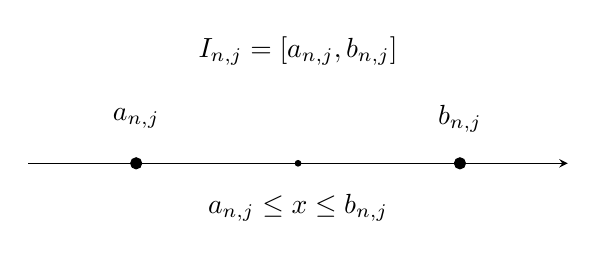
\begin{tikzpicture}
      \begin{axis}[
          xmin=-10, xmax=10,
          axis x line=center,
          hide y axis,
          ymin=-5,ymax=5,
          xtick=\empty,
          xticklabels=\empty,
        ]
        \draw[color=black] (0,2.5) node {$I_{n,j} = [a_{n,j}, b_{n,j}]$};
        \begin{scriptsize}
          \draw [fill=black] (-6,0) circle (2pt);
          \draw[color=black] (-6,1) node {$a_{n,j}$};

          \draw [fill=black] (0,0) circle (1pt);
          \draw[color=black] (0,-1) node {$a_{n,j} \le x \le b_{n,j}$};

          \draw [fill=black] (6,0) circle (2pt);
          \draw[color=black] (6,1) node {$b_{n,j}$};
        \end{scriptsize}
      \end{axis}
    \end{tikzpicture}

    \[\cdots\]
  \end{center}
  对于每个 $j$ 而言都满足 Theorem 2.38,因此证明中所给的某实数集 $x_j^*\ (1 \le j \le k)$ 也满足定理。
\end{anote}

\begin{theorem}
  Every $k$-cell is compact.
\end{theorem}

\begin{proof}
  令 $I$ 为一个 $k$-方格,由所有点 $\mathbf{x}=(x_1,\dots,x_k)$ 构成,使得 $a_j \le x_j \le b_j \ (1 \le j \le k)$。令
  \[\delta = \biggl\{\sum_{1}^{k}(b_j - a_j)^2\biggr\}^{1/2}\]
  那么 $|\mathbf{x} - \mathbf{y}| \le \delta$,如果 $\mathbf{x} \in I,\ \mathbf{y} \in I$。

  假设为了得到一个悖论,存在一个 $I$ 的开覆盖 $\{G_{\alpha}\}$ 不包含 $I$ 的有限子覆盖。令 $c_j = (a_j + b_j) / 2$。
  那么区间 $[a_j, c_j]$ 以及 $[c_j, b_j]$ 决定了 $2^k$ $k$-方格 $Q_i$ 的并集为 $I$。在 $Q_i$ 中至少有一个称为 $I_1$ 的集合,
  不能被 $\{G_{\alpha}\}$ 的任何有限子类覆盖(否则 $I$ 就被覆盖了)。接下来再细分 $I_1$ 并继续上述步骤。我们获得一个具有以下属性
  的数列 $\{I_n\}$ :
  \begin{enumerate}[label=(\alph*)]
    \item $I \supset I_1 \supset I_2 \supset I_3 \supset \cdots$;
    \item $I_n$ 没有被 $\{G_{\alpha}\}$ 任何的有限子类覆盖;
    \item 如果 $\mathbf{x} \in I_n$ 且 $\mathbf{y} \in I_n$,那么 $|\mathbf{x} - \mathbf{y}| \le 2^{-n} \delta$。
  \end{enumerate}

  通过 (a) 与 Theorem 2.39 可知,点 $\mathbf{x}^*$ 存在于每个 $I_n$ 中。对于某些 $\alpha$ 有 $\mathbf{x}^* \in G_{\alpha}$。
  因为 $\{G_{\alpha}\}$ 是开的,存在 $r>0$ 使得 $|\mathbf{y} - \mathbf{x}^*| < r$ 推导出 $\mathbf{y} \in G_{\alpha}$。
  如果 $n$ 很大使得 $2^{-n}\delta<r$(这个 $n$ 是存在的,否则对于所有正整数 $n$ 有 $2^{n} \le \delta/r$,这就与有理数 $R$ 的
  阿基米德性质相悖),那么 (c) 意为 $I_n \subset G_{\alpha}$,即与 (b) 相悖。

  证明完成。
\end{proof}

下一个定理中的与 (a) 和 (b) 相等部分又被称作海涅-博雷尔定理 Heine–Borel theorem。

\begin{anote}
  简单来说 $1 \le j \le k$ 的 $j$ 代表着每个维度,那么其所设定的 $a_j \le x_j \le b_j$ 可视为每个维度都有\say{闭区间}对 $x$ 进行约束。
  那么 $\delta = \Bigl\{\sum\limits_1^k(b_j-a_j)^2\Bigr\}^{1/2}$ 很明显就是一个距离公式(例如二维情况下的
  $d = \sqrt{(x_1-x_2)^2 + (y_1-y_2)^2}$)。那么对于任意 $\mathbf{x},\ \mathbf{y}\in I$ 有 $|\mathbf{x}-\mathbf{y}|\le\delta$
  的意思就是任意两点之间的距离永远小于等于这个最大边界范围 $\delta$。

  那么为了证明 $k$-方格是紧的,可以利用紧性的定理来做悖论的假设,即假设 $I$ 不存在有限个开覆盖。随后的\say{determine $2^k$ $k$-cells}
  看起来比较抽象,但是从其设定的 $c_j=(a_j + b_j)/2$ 可以看的出来 $c_j$ 是 $a_j$ 与 $b_j$ 的中点。那么 $c_j$ 所分隔的\say{两边} 为
  $[a_j,c_j]$ 与 $[c_j,b_j]$ 构成了 $2^k$ 个 $k$-方格(带入到一维空间就是分隔成了两个线段,而带入到二维则是被分隔成四个象限,
  三维则是八个象限)。那么对于 $2^k$ 的 $k$-方格而言,设其为 $Q_i$,而其本质还是 $I$,因此说 $Q_i$ 的并集为 $I$。为了得到悖论,
  将其中一个称为 $I_1$ 的 $Q_i$,假设为不紧的,即不存在有限的子覆盖。接下来就是对该 $I_1$ 进行分解,利用了 Theorem 2.39 的结论将其转换为
  数列 $\{I_n\}$ 并附上证明中的三个性质。由 (a) 和 Theorem 2.39 得出总有 $\mathbf{x^*} \in G_{\alpha}$。而因为 $G_{\alpha}$ 是开集,
  总会有 $r>0$ 使得 $|\mathbf{y}-\mathbf{x}^*|<r$,所以 $\mathbf{y} \in G$。

  这其中 (c) 的 $|\mathbf{x}-\mathbf{y}|\le2^{-n}\delta$ 可视为在 $I_n$ 中的两点,它们之间的距离小于 $\frac{1}{2^n} \delta$。
  这里最简单的几何理解就是在一维空间下的:
  \begin{center}
    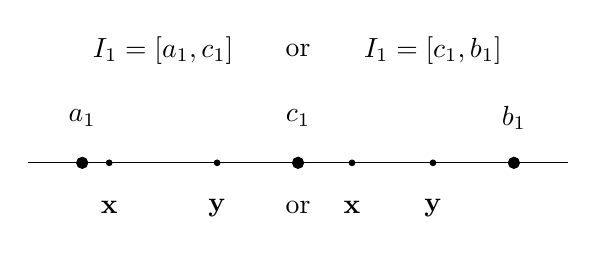
\begin{tikzpicture}
      \begin{axis}[
          xmin=-10, xmax=10,
          axis x line*=middle,
          hide y axis,
          ymin=-5,ymax=5,
          xtick=\empty,
          xticklabels=\empty,
        ]
        \draw[color=black] (-5,2.5) node {$I_1 = [a_1, c_1]$};
        \draw[color=black] (0,2.5) node {or};
        \draw[color=black] (5,2.5) node {$I_1 = [c_1, b_1]$};
        \draw[color=black] (0,-1) node {or};
        \begin{scriptsize}
          \draw [fill=black] (-8,0) circle (2pt);
          \draw[color=black] (-8,1) node {$a_1$};

          \draw [fill=black] (-7,0) circle (1pt);
          \draw[color=black] (-7,-1) node {$\mathbf{x}$};

          \draw [fill=black] (-3,0) circle (1pt);
          \draw[color=black] (-3,-1) node {$\mathbf{y}$};

          \draw [fill=black] (0,0) circle (2pt);
          \draw[color=black] (0,1) node {$c_1$};

          \draw [fill=black] (2,0) circle (1pt);
          \draw[color=black] (2,-1) node {$\mathbf{x}$};

          \draw [fill=black] (5,0) circle (1pt);
          \draw[color=black] (5,-1) node {$\mathbf{y}$};

          \draw [fill=black] (8,0) circle (2pt);
          \draw[color=black] (8,1) node {$b_1$};
        \end{scriptsize}
      \end{axis}
    \end{tikzpicture}
  \end{center}
  也就是说,根据之前 $c_j$ 的分隔动作,将 $I$ 分成了 $2^1$ 个 $1$-方格的 $Q_i$。那么证明中说的至少其中一个不会被 $\{G_{\alpha}\}$ 中任何有限的
  子类所覆盖,那么如图所示,$I_1$ 要么是在左侧的 $[a_1,c_1]$ 处,要么是在右侧的 $[c_1,b_1]$ 处。因此图示中 $\mathbf{x}$ 与 $\mathbf{y}$
  的距离要小于等于 $\delta/2$,即小于 $\frac{|b_1-a_1|}{2}$。

  之后根据第一章的阿基米德性质\say{给出任何正数,总能够挑选出一个整数其倒数小过原来的数},可以很轻松的得出 (c) 与 (b) 相悖。
\end{anote}

\begin{theorem}
  If a set $E$ in $R^k$ has one of the following three properties, then it has the other two:
  \begin{enumerate}[label=(\alph*)]
    \item $E$ is closed and bounded.
    \item $E$ is compact.
    \item Every infinite subset of $E$ has a limit point in $E$.
  \end{enumerate}
\end{theorem}

\begin{proof}
  如果 (a) 成立,那么对于一些$k$-方格有 $E \subset I$,那么 (b) 遵循 Theorems 2.40 与 2.34。Theorem 2.37 展示 (b) 推导 (c)。
  现在剩下 (c) 如何推导 (a)。

  如果 $E$ 没有边界,那么 $E$ 包含了点 $\mathbf{x}_n$ 且
  \[|\mathbf{x}_n| > n \quad (n=1,2,3,\dots)\]
  由这些点 $\mathbf{x}_n$ 构成的集合 $S$ 是无限的,且明显在 $R^k$ 中没有极限点,因此在 $E$ 中也不存在极限点。因此 (c) 推导出
  $E$ 是有界的。

  如果 $E$ 不是闭的,那么存在一个点 $\mathbf{x}_0 \in R^k$ 是 $E$ 的极限点且不在 $E$ 中。 对于 $n=1,2,3,\dots$ 存在点
  $\mathbf{x}_n \in E$ 使得 $|\mathbf{x}_n - \mathbf{x}_0| < 1/n$。令 $S$ 成为这些点 $\mathbf{x}_n$ 的集合。那么 $S$ 是
  无限的(否则 $|\mathbf{x}_n - \mathbf{x}_0|$ 将有一个常量正数,对于无限多的 $n$),$S$ 拥有 $\mathbf{x}_0$ 作为一个极限点,
  且 $S$ 没有其他的极限点在 $R^k$ 中。那么如果 $\mathbf{y} \in R^k, \ \mathbf{y} \ne \mathbf{x}_0$,则
  \begin{align*}
    \mathcal{} |\mathbf{x}_n - \mathbf{y}| & \ge |\mathbf{x}_0 - \mathbf{y}| - |\mathbf{x}_n - \mathbf{x}_0| \\
                                           & \ge |\mathbf{x}_0 - \mathbf{y}| - \frac{1}{n}                   \\
                                           & \ge \frac{1}{2}|\mathbf{x}_0 - \mathbf{y}|
  \end{align*}
  满足所有且有限多的 $n$;这证明 $\mathbf{y}$ 不是 $S$ 的极限点(Theorem 2.20)。

  因此 $S$ 在 $E$ 中没有极限点;因此如果 (c) 成立,那么 $E$ 必须是闭的。
\end{proof}

值得注意,这里的 (b) 和 (c) 等同于任何度量空间;但是 (a) 不是,通常来说用于推导 (b) 与 (c)。

\begin{theorem}[Weierstrass]
  Every bounded infinite subset of $R^k$ has a limit point in $R^k$.
\end{theorem}

\begin{proof}
  因为有界,集合 $E$ 是 $k$-方格 $I \subset R^k$ 的一个子集。根据 Theorem 2.40,$I$ 是紧的,因此根据 Theorem 2.37, $E$ 在
  $I$ 中拥有一个极限点。
\end{proof}

\end{document}
